% Options for packages loaded elsewhere
\PassOptionsToPackage{unicode}{hyperref}
\PassOptionsToPackage{hyphens}{url}
%
\documentclass[
]{article}
\usepackage{amsmath,amssymb}
\usepackage{lmodern}
\usepackage{iftex}
\ifPDFTeX
  \usepackage[T1]{fontenc}
  \usepackage[utf8]{inputenc}
  \usepackage{textcomp} % provide euro and other symbols
\else % if luatex or xetex
  \usepackage{unicode-math}
  \defaultfontfeatures{Scale=MatchLowercase}
  \defaultfontfeatures[\rmfamily]{Ligatures=TeX,Scale=1}
\fi
% Use upquote if available, for straight quotes in verbatim environments
\IfFileExists{upquote.sty}{\usepackage{upquote}}{}
\IfFileExists{microtype.sty}{% use microtype if available
  \usepackage[]{microtype}
  \UseMicrotypeSet[protrusion]{basicmath} % disable protrusion for tt fonts
}{}
\makeatletter
\@ifundefined{KOMAClassName}{% if non-KOMA class
  \IfFileExists{parskip.sty}{%
    \usepackage{parskip}
  }{% else
    \setlength{\parindent}{0pt}
    \setlength{\parskip}{6pt plus 2pt minus 1pt}}
}{% if KOMA class
  \KOMAoptions{parskip=half}}
\makeatother
\usepackage{xcolor}
\usepackage[margin=1in]{geometry}
\usepackage{color}
\usepackage{fancyvrb}
\newcommand{\VerbBar}{|}
\newcommand{\VERB}{\Verb[commandchars=\\\{\}]}
\DefineVerbatimEnvironment{Highlighting}{Verbatim}{commandchars=\\\{\}}
% Add ',fontsize=\small' for more characters per line
\usepackage{framed}
\definecolor{shadecolor}{RGB}{248,248,248}
\newenvironment{Shaded}{\begin{snugshade}}{\end{snugshade}}
\newcommand{\AlertTok}[1]{\textcolor[rgb]{0.94,0.16,0.16}{#1}}
\newcommand{\AnnotationTok}[1]{\textcolor[rgb]{0.56,0.35,0.01}{\textbf{\textit{#1}}}}
\newcommand{\AttributeTok}[1]{\textcolor[rgb]{0.77,0.63,0.00}{#1}}
\newcommand{\BaseNTok}[1]{\textcolor[rgb]{0.00,0.00,0.81}{#1}}
\newcommand{\BuiltInTok}[1]{#1}
\newcommand{\CharTok}[1]{\textcolor[rgb]{0.31,0.60,0.02}{#1}}
\newcommand{\CommentTok}[1]{\textcolor[rgb]{0.56,0.35,0.01}{\textit{#1}}}
\newcommand{\CommentVarTok}[1]{\textcolor[rgb]{0.56,0.35,0.01}{\textbf{\textit{#1}}}}
\newcommand{\ConstantTok}[1]{\textcolor[rgb]{0.00,0.00,0.00}{#1}}
\newcommand{\ControlFlowTok}[1]{\textcolor[rgb]{0.13,0.29,0.53}{\textbf{#1}}}
\newcommand{\DataTypeTok}[1]{\textcolor[rgb]{0.13,0.29,0.53}{#1}}
\newcommand{\DecValTok}[1]{\textcolor[rgb]{0.00,0.00,0.81}{#1}}
\newcommand{\DocumentationTok}[1]{\textcolor[rgb]{0.56,0.35,0.01}{\textbf{\textit{#1}}}}
\newcommand{\ErrorTok}[1]{\textcolor[rgb]{0.64,0.00,0.00}{\textbf{#1}}}
\newcommand{\ExtensionTok}[1]{#1}
\newcommand{\FloatTok}[1]{\textcolor[rgb]{0.00,0.00,0.81}{#1}}
\newcommand{\FunctionTok}[1]{\textcolor[rgb]{0.00,0.00,0.00}{#1}}
\newcommand{\ImportTok}[1]{#1}
\newcommand{\InformationTok}[1]{\textcolor[rgb]{0.56,0.35,0.01}{\textbf{\textit{#1}}}}
\newcommand{\KeywordTok}[1]{\textcolor[rgb]{0.13,0.29,0.53}{\textbf{#1}}}
\newcommand{\NormalTok}[1]{#1}
\newcommand{\OperatorTok}[1]{\textcolor[rgb]{0.81,0.36,0.00}{\textbf{#1}}}
\newcommand{\OtherTok}[1]{\textcolor[rgb]{0.56,0.35,0.01}{#1}}
\newcommand{\PreprocessorTok}[1]{\textcolor[rgb]{0.56,0.35,0.01}{\textit{#1}}}
\newcommand{\RegionMarkerTok}[1]{#1}
\newcommand{\SpecialCharTok}[1]{\textcolor[rgb]{0.00,0.00,0.00}{#1}}
\newcommand{\SpecialStringTok}[1]{\textcolor[rgb]{0.31,0.60,0.02}{#1}}
\newcommand{\StringTok}[1]{\textcolor[rgb]{0.31,0.60,0.02}{#1}}
\newcommand{\VariableTok}[1]{\textcolor[rgb]{0.00,0.00,0.00}{#1}}
\newcommand{\VerbatimStringTok}[1]{\textcolor[rgb]{0.31,0.60,0.02}{#1}}
\newcommand{\WarningTok}[1]{\textcolor[rgb]{0.56,0.35,0.01}{\textbf{\textit{#1}}}}
\usepackage{graphicx}
\makeatletter
\def\maxwidth{\ifdim\Gin@nat@width>\linewidth\linewidth\else\Gin@nat@width\fi}
\def\maxheight{\ifdim\Gin@nat@height>\textheight\textheight\else\Gin@nat@height\fi}
\makeatother
% Scale images if necessary, so that they will not overflow the page
% margins by default, and it is still possible to overwrite the defaults
% using explicit options in \includegraphics[width, height, ...]{}
\setkeys{Gin}{width=\maxwidth,height=\maxheight,keepaspectratio}
% Set default figure placement to htbp
\makeatletter
\def\fps@figure{htbp}
\makeatother
\setlength{\emergencystretch}{3em} % prevent overfull lines
\providecommand{\tightlist}{%
  \setlength{\itemsep}{0pt}\setlength{\parskip}{0pt}}
\setcounter{secnumdepth}{-\maxdimen} % remove section numbering
\ifLuaTeX
  \usepackage{selnolig}  % disable illegal ligatures
\fi
\IfFileExists{bookmark.sty}{\usepackage{bookmark}}{\usepackage{hyperref}}
\IfFileExists{xurl.sty}{\usepackage{xurl}}{} % add URL line breaks if available
\urlstyle{same} % disable monospaced font for URLs
\hypersetup{
  pdftitle={Lösung Zettel 2},
  hidelinks,
  pdfcreator={LaTeX via pandoc}}

\title{Lösung Zettel 2}
\author{}
\date{\vspace{-2.5em}2023-06-01}

\begin{document}
\maketitle

\hypertarget{aufgabe-1}{%
\subsection{Aufgabe 1}\label{aufgabe-1}}

Lade zun ̈achst den Datenrahmen df spacebar aus dem Paket
\texttt{bcogsci}.

\begin{Shaded}
\begin{Highlighting}[]
\FunctionTok{library}\NormalTok{(bcogsci)}
\FunctionTok{data}\NormalTok{(}\StringTok{"df\_spacebar"}\NormalTok{)}
\end{Highlighting}
\end{Shaded}

\begin{center}\rule{0.5\linewidth}{0.5pt}\end{center}

\hypertarget{a}{%
\paragraph{a)}\label{a}}

Es ist immer eine gute Idee, Daten grafisch darzustellen, bevor man
etwas anderes tut; plotte die Daten. (Unsere Response ist ''t'').

\hypertarget{luxf6sungsansatz}{%
\paragraph{Lösungsansatz:}\label{luxf6sungsansatz}}

\begin{itemize}
\tightlist
\item
  Histogram der Response Variable
\item
  Line/Dot-Plot der Daten
\end{itemize}

\begin{Shaded}
\begin{Highlighting}[]
\FunctionTok{par}\NormalTok{(}\AttributeTok{mfrow =} \FunctionTok{c}\NormalTok{(}\DecValTok{1}\NormalTok{, }\DecValTok{2}\NormalTok{)) }\CommentTok{\# zwei Grafiken in einer Figure}
\FunctionTok{hist}\NormalTok{(df\_spacebar}\SpecialCharTok{$}\NormalTok{t)}
\FunctionTok{plot}\NormalTok{(df\_spacebar}\SpecialCharTok{$}\NormalTok{t)}
\end{Highlighting}
\end{Shaded}

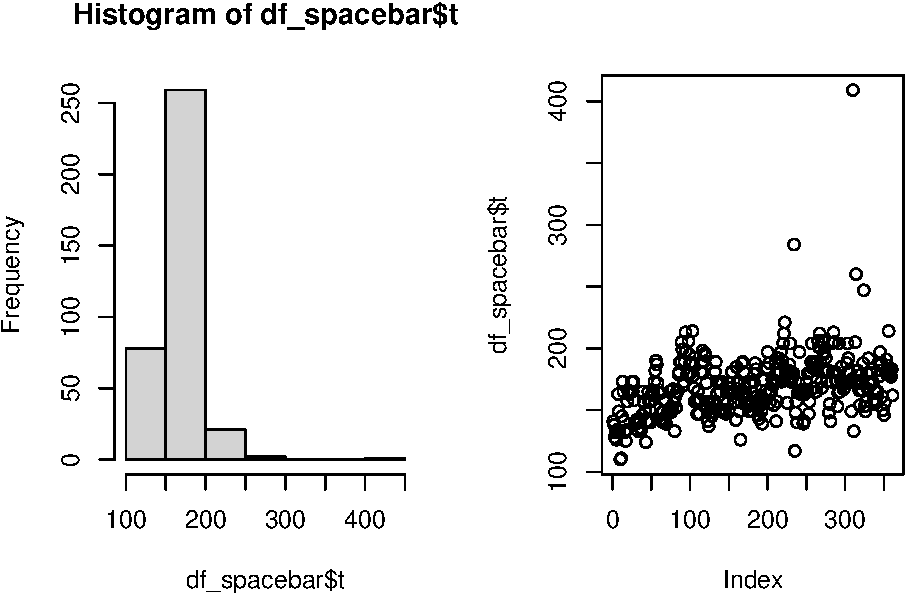
\includegraphics{Loesung-Zettel-2_files/figure-latex/loesung_a-1.pdf}

\begin{center}\rule{0.5\linewidth}{0.5pt}\end{center}

\hypertarget{b}{%
\paragraph{b)}\label{b}}

Fitte ein Intercept Model auf den Daten mit Hilfe des brms Packages. t
sei dabei die Response. Die Angenommene Verteilungsfamilie für t ist die
Normalverteilung (\texttt{gaussian()}). Unterstelle erst einmal
uninformative Prior: Für den Intercept \(Uniform(0, 600)\) und Sigma
\(Uniform(0, 20)\). Setze die Iterationen auf 50 und das warumup auf 25.
Konvergiert das Model? Woran erkennst du es?
\textit{Hint: Anhand des R Outputs und eines Model Plots.}

\hypertarget{luxf6sungsansatz-1}{%
\paragraph{Lösungsansatz:}\label{luxf6sungsansatz-1}}

\begin{Shaded}
\begin{Highlighting}[]
\NormalTok{df\_spacebar\_new }\OtherTok{=}\NormalTok{ df\_spacebar}
\NormalTok{df\_spacebar\_new}\SpecialCharTok{$}\NormalTok{t }\OtherTok{\textless{}{-}}\NormalTok{ (df\_spacebar\_new}\SpecialCharTok{$}\NormalTok{t)}\SpecialCharTok{/}\DecValTok{10}
\NormalTok{model\_b }\OtherTok{=} \FunctionTok{brm}\NormalTok{(t }\SpecialCharTok{\textasciitilde{}} \DecValTok{1}\NormalTok{,    }\CommentTok{\# Intercept: 1}
              \AttributeTok{family =} \FunctionTok{gaussian}\NormalTok{(),}
              \AttributeTok{prior =}
                  \FunctionTok{c}\NormalTok{(}
                    \FunctionTok{prior}\NormalTok{(}\FunctionTok{uniform}\NormalTok{(}\DecValTok{0}\NormalTok{,}\DecValTok{600}\NormalTok{), }\AttributeTok{lb =} \DecValTok{0}\NormalTok{, }\AttributeTok{ub =} \DecValTok{600}\NormalTok{, }\AttributeTok{class =}\NormalTok{ Intercept),}
                    \FunctionTok{prior}\NormalTok{(}\FunctionTok{uniform}\NormalTok{(}\DecValTok{0}\NormalTok{,}\DecValTok{20}\NormalTok{), }\AttributeTok{lb =} \DecValTok{0}\NormalTok{, }\AttributeTok{ub =} \DecValTok{20}\NormalTok{, }\AttributeTok{class =}\NormalTok{ sigma)}
\NormalTok{                  ),}
              \AttributeTok{warmup =} \DecValTok{25}\NormalTok{,}
              \AttributeTok{iter =} \DecValTok{50}\NormalTok{,}
                \AttributeTok{data =}\NormalTok{ df\_spacebar}
\NormalTok{              )}
\end{Highlighting}
\end{Shaded}

Model Ergebnisse anschauen

\begin{Shaded}
\begin{Highlighting}[]
\NormalTok{model\_b}
\end{Highlighting}
\end{Shaded}

\begin{verbatim}
## Warning: Parts of the model have not converged (some Rhats are > 1.05). Be
## careful when analysing the results! We recommend running more iterations and/or
## setting stronger priors.
\end{verbatim}

\begin{verbatim}
##  Family: gaussian 
##   Links: mu = identity; sigma = identity 
## Formula: t ~ 1 
##    Data: df_spacebar (Number of observations: 361) 
##   Draws: 4 chains, each with iter = 50; warmup = 25; thin = 1;
##          total post-warmup draws = 100
## 
## Population-Level Effects: 
##           Estimate Est.Error l-95% CI u-95% CI Rhat Bulk_ESS Tail_ESS
## Intercept   168.85      0.84   167.46   170.55 1.02      182       94
## 
## Family Specific Parameters: 
##       Estimate Est.Error l-95% CI u-95% CI Rhat Bulk_ESS Tail_ESS
## sigma    18.06      2.04    14.23    19.99 2.87        7       14
## 
## Draws were sampled using sampling(NUTS). For each parameter, Bulk_ESS
## and Tail_ESS are effective sample size measures, and Rhat is the potential
## scale reduction factor on split chains (at convergence, Rhat = 1).
\end{verbatim}

Analyse des Models

\begin{Shaded}
\begin{Highlighting}[]
\FunctionTok{plot}\NormalTok{(model\_b)}
\end{Highlighting}
\end{Shaded}

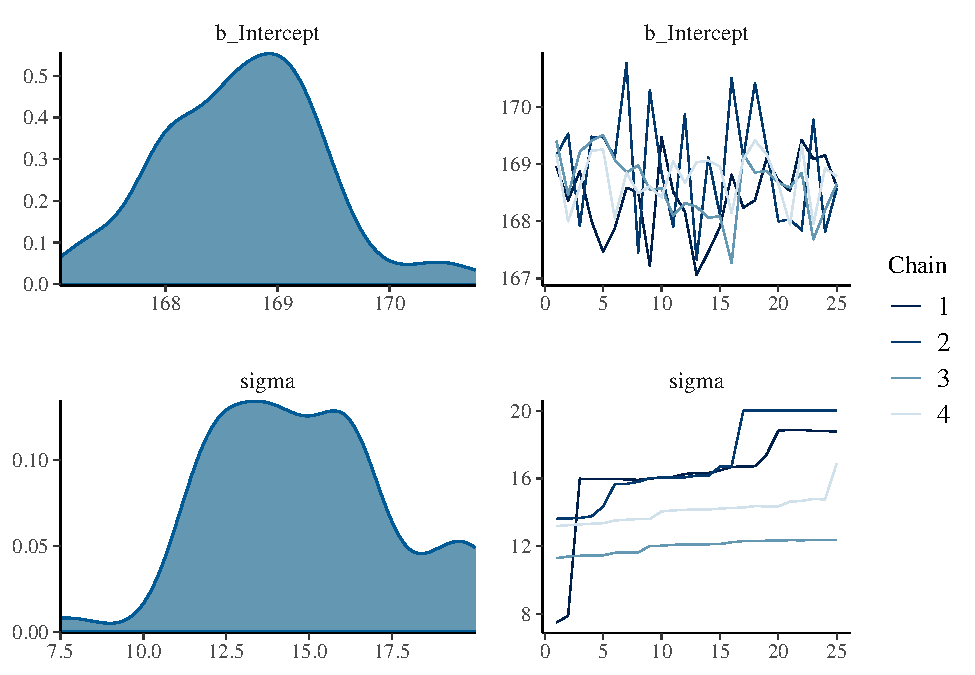
\includegraphics{Loesung-Zettel-2_files/figure-latex/unnamed-chunk-2-1.pdf}

Wir sehen hier ein Problem mit den ``Catapilar'' Plots. Die Graphen
liegen nicht übereinander. Es bedeutet, dass wir hier keine Konvergenz
beobachten. Die Anzahl der Iterationen reicht scheinbar nicht aus.

\begin{center}\rule{0.5\linewidth}{0.5pt}\end{center}

\hypertarget{c}{%
\paragraph{c)}\label{c}}

Fitte das gleiche Modell, verändere nur die Anzahl der Iterationen auf
2000 und die Warmup auf 1000. Unterstelle für den Intercept einen Prior
\(Uniform(0, 60000)\) und einen Sigma Pior \(Uniform(0, 2000)\).
Konvergiert das Model? Woran machst du diese Entscheidung fest?

\hypertarget{luxf6sungsansatz-2}{%
\paragraph{Lösungsansatz:}\label{luxf6sungsansatz-2}}

\begin{Shaded}
\begin{Highlighting}[]
\NormalTok{model\_c }\OtherTok{=} \FunctionTok{brm}\NormalTok{(t }\SpecialCharTok{\textasciitilde{}} \DecValTok{1}\NormalTok{,    }\CommentTok{\# Intercept: 1}
              \AttributeTok{family =} \FunctionTok{gaussian}\NormalTok{(),}
              \AttributeTok{prior =}
                  \FunctionTok{c}\NormalTok{(}
                    \FunctionTok{prior}\NormalTok{(}\FunctionTok{uniform}\NormalTok{(}\DecValTok{0}\NormalTok{,}\DecValTok{600}\NormalTok{), }\AttributeTok{lb =} \DecValTok{0}\NormalTok{, }\AttributeTok{ub =} \DecValTok{600}\NormalTok{, }\AttributeTok{class =}\NormalTok{ Intercept),}
                    \FunctionTok{prior}\NormalTok{(}\FunctionTok{uniform}\NormalTok{(}\DecValTok{0}\NormalTok{,}\DecValTok{20}\NormalTok{), }\AttributeTok{lb =} \DecValTok{0}\NormalTok{, }\AttributeTok{ub =} \DecValTok{20}\NormalTok{, }\AttributeTok{class =}\NormalTok{ sigma)}
\NormalTok{                  ),}
                \AttributeTok{data =}\NormalTok{ df\_spacebar}
\NormalTok{              )}
\end{Highlighting}
\end{Shaded}

Model Ergebnisse anschauen

\begin{Shaded}
\begin{Highlighting}[]
\NormalTok{model\_c}
\end{Highlighting}
\end{Shaded}

\begin{verbatim}
##  Family: gaussian 
##   Links: mu = identity; sigma = identity 
## Formula: t ~ 1 
##    Data: df_spacebar (Number of observations: 361) 
##   Draws: 4 chains, each with iter = 2000; warmup = 1000; thin = 1;
##          total post-warmup draws = 4000
## 
## Population-Level Effects: 
##           Estimate Est.Error l-95% CI u-95% CI Rhat Bulk_ESS Tail_ESS
## Intercept   168.67      1.02   166.71   170.64 1.00     2491     2237
## 
## Family Specific Parameters: 
##       Estimate Est.Error l-95% CI u-95% CI Rhat Bulk_ESS Tail_ESS
## sigma    19.91      0.09    19.66    20.00 1.00     1918     1391
## 
## Draws were sampled using sampling(NUTS). For each parameter, Bulk_ESS
## and Tail_ESS are effective sample size measures, and Rhat is the potential
## scale reduction factor on split chains (at convergence, Rhat = 1).
\end{verbatim}

Analyse des Models

\begin{Shaded}
\begin{Highlighting}[]
\FunctionTok{plot}\NormalTok{(model\_c)}
\end{Highlighting}
\end{Shaded}

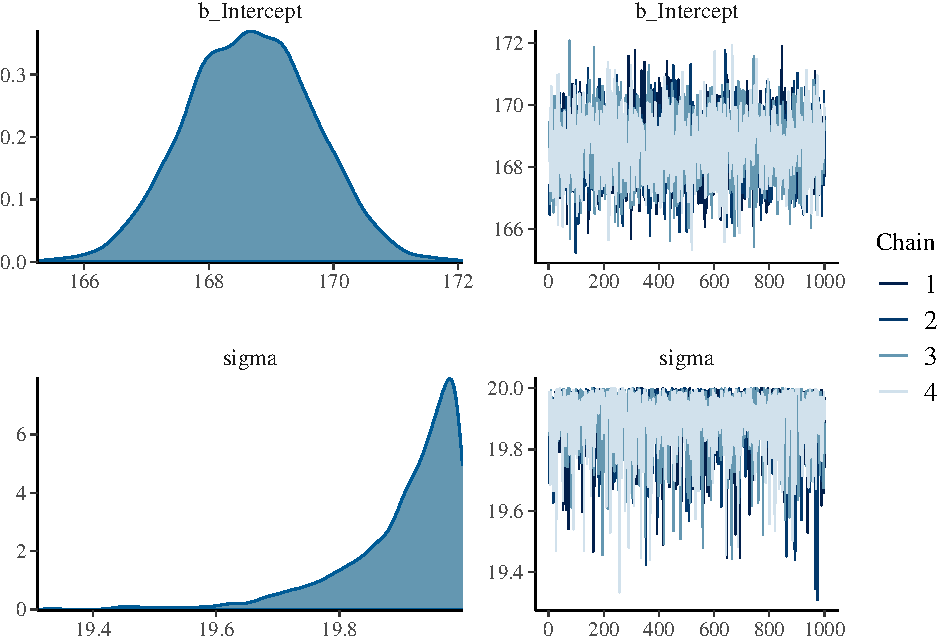
\includegraphics{Loesung-Zettel-2_files/figure-latex/unnamed-chunk-4-1.pdf}

Wir beobachten Konvergenz! Allerdings sehen wir, dass der Prior für das
Sigma vielleicht nicht wirklich gut gewählt worden ist.

\begin{center}\rule{0.5\linewidth}{0.5pt}\end{center}

\hypertarget{d}{%
\paragraph{d)}\label{d}}

Wähle unter Berücksichtigung von Normalverteilung der Daten, einen Prior
der besser zu den Daten passt. Überlege einen vernünftigen Satz von
Prior für \(\mu\) und \(\sigma\). Begründe wie du auf diese Auswahl
kommst. Es gibt hier keine richtige Antwort!
\textit{Die Grafik aus a) kann euch helfen einen Entscheidung zu treffen.}

\hypertarget{luxf6sungsansatz-3}{%
\paragraph{Lösungsansatz:}\label{luxf6sungsansatz-3}}

\begin{itemize}
\tightlist
\item
  Wir beobachten keine negativen Werte.
\item
\end{itemize}

\begin{Shaded}
\begin{Highlighting}[]
\FunctionTok{summary}\NormalTok{(df\_spacebar}\SpecialCharTok{$}\NormalTok{t)}
\end{Highlighting}
\end{Shaded}

\begin{verbatim}
##    Min. 1st Qu.  Median    Mean 3rd Qu.    Max. 
##   110.0   156.0   166.0   168.6   181.0   409.0
\end{verbatim}

\begin{Shaded}
\begin{Highlighting}[]
\FunctionTok{mean}\NormalTok{(df\_spacebar}\SpecialCharTok{$}\NormalTok{t); }\FunctionTok{sd}\NormalTok{(df\_spacebar}\SpecialCharTok{$}\NormalTok{t)}
\end{Highlighting}
\end{Shaded}

\begin{verbatim}
## [1] 168.6399
\end{verbatim}

\begin{verbatim}
## [1] 24.9118
\end{verbatim}

\begin{Shaded}
\begin{Highlighting}[]
\NormalTok{model\_d }\OtherTok{=} \FunctionTok{brm}\NormalTok{(t }\SpecialCharTok{\textasciitilde{}} \DecValTok{1}\NormalTok{,    }\CommentTok{\# Intercept: 1}
              \AttributeTok{family =} \FunctionTok{gaussian}\NormalTok{(),}
              \AttributeTok{prior =}
                  \FunctionTok{c}\NormalTok{(}
                    \FunctionTok{prior}\NormalTok{(}\FunctionTok{normal}\NormalTok{(}\DecValTok{168}\NormalTok{,}\DecValTok{30}\NormalTok{), }\AttributeTok{class =}\NormalTok{ Intercept),}
                    \FunctionTok{prior}\NormalTok{(}\FunctionTok{normal}\NormalTok{(}\DecValTok{0}\NormalTok{,}\DecValTok{30}\NormalTok{), }\AttributeTok{class =}\NormalTok{ sigma)}
\NormalTok{                  ),}
                \AttributeTok{data =}\NormalTok{ df\_spacebar}
\NormalTok{              )}
\end{Highlighting}
\end{Shaded}

\begin{Shaded}
\begin{Highlighting}[]
\NormalTok{model\_d}
\end{Highlighting}
\end{Shaded}

\begin{verbatim}
##  Family: gaussian 
##   Links: mu = identity; sigma = identity 
## Formula: t ~ 1 
##    Data: df_spacebar (Number of observations: 361) 
##   Draws: 4 chains, each with iter = 2000; warmup = 1000; thin = 1;
##          total post-warmup draws = 4000
## 
## Population-Level Effects: 
##           Estimate Est.Error l-95% CI u-95% CI Rhat Bulk_ESS Tail_ESS
## Intercept   168.62      1.32   166.09   171.19 1.00     3760     2580
## 
## Family Specific Parameters: 
##       Estimate Est.Error l-95% CI u-95% CI Rhat Bulk_ESS Tail_ESS
## sigma    24.98      0.92    23.33    26.95 1.00     3716     2514
## 
## Draws were sampled using sampling(NUTS). For each parameter, Bulk_ESS
## and Tail_ESS are effective sample size measures, and Rhat is the potential
## scale reduction factor on split chains (at convergence, Rhat = 1).
\end{verbatim}

Analyse des Models

\begin{Shaded}
\begin{Highlighting}[]
\FunctionTok{plot}\NormalTok{(model\_d)}
\end{Highlighting}
\end{Shaded}

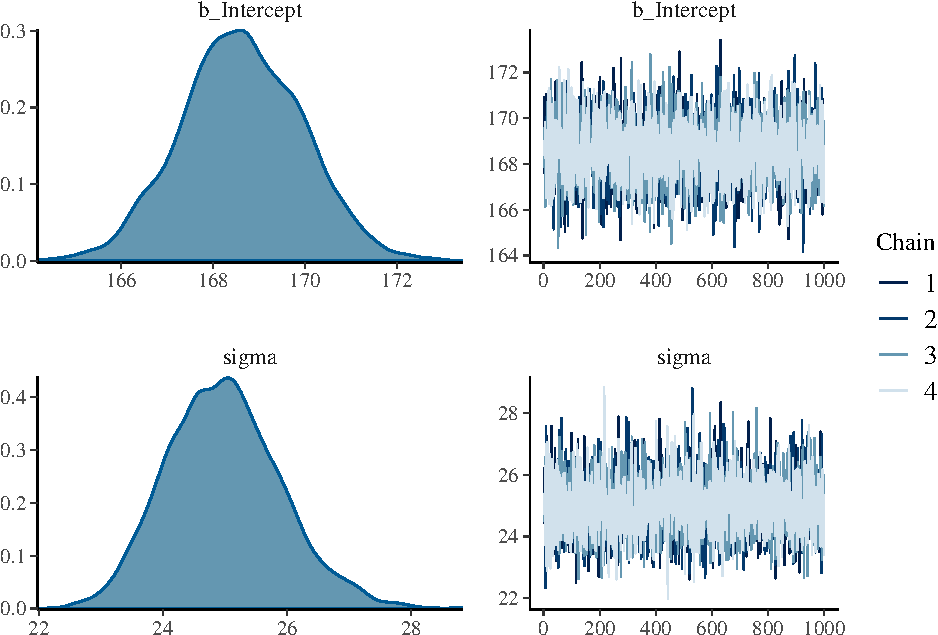
\includegraphics{Loesung-Zettel-2_files/figure-latex/unnamed-chunk-7-1.pdf}

\begin{center}\rule{0.5\linewidth}{0.5pt}\end{center}

\hypertarget{e}{%
\paragraph{e)}\label{e}}

Nutze die von dir aufgestellten Prior um das neue Model zu fitten. Wenn
du die Modellergebnisse vergleichst was fällt dir auf?
\textit{Hint: die summary() des Modells ist immer ein guter Startpunkt.}

\hypertarget{luxf6sungsansatz-4}{%
\paragraph{Lösungsansatz:}\label{luxf6sungsansatz-4}}

\begin{center}\rule{0.5\linewidth}{0.5pt}\end{center}

\hypertarget{f}{%
\paragraph{f)}\label{f}}

Kannst du aussagekräftige Priors finden, die den Posterior in spürbarer
Weise beeinflussen ? (verwende Normalverteilungen für Priors, keine
gleichmäßigen Priors) Auch hier gibt es keine richtigen Antworten.
Möglicherweise musst du mehrere verschiedene Priors ausprobieren, bevor
du den Posterior merklich beeinflussen können.
\textit{Wiederholung: Aussagekräfte Prior: Prior die ''Wissen'' in die Analyse bringen. Z.B Weißt du vorher schon wo der Mittelwert sein müsste? Wie ist die Varianz?}

\hypertarget{luxf6sungsansatz-5}{%
\paragraph{Lösungsansatz:}\label{luxf6sungsansatz-5}}

\begin{center}\rule{0.5\linewidth}{0.5pt}\end{center}

\hypertarget{g}{%
\paragraph{g)}\label{g}}

Erzeuge auf der Grundlage dieses neuen Priors ein Modell und zeige die
Posterior Predictive Verteilungen und plotte sie.
\textit{Tipp: Das R-Package bayesplot hat nützliche Funktionen.}

\hypertarget{luxf6sungsansatz-6}{%
\paragraph{Lösungsansatz:}\label{luxf6sungsansatz-6}}

\end{document}
